\documentclass{article}

\usepackage[utf8x]{inputenc}
\usepackage[english,russian]{babel}
\usepackage{cmap}
\usepackage{commath}
\usepackage{amsmath}
\usepackage{amsfonts}
\usepackage{mathtools}
\usepackage{amssymb}
\usepackage{parskip}
\usepackage{titling}
\usepackage{color}
\usepackage{hyperref}
\usepackage{cancel}
\usepackage{enumerate}
\usepackage{multicol}
\usepackage{graphicx}
\usepackage[font=small,labelfont=bf]{caption}
\usepackage[a4paper, left=2.5cm, right=1.5cm, top=2.5cm, bottom=2.5cm]{geometry}

\graphicspath{ {./images/} }
\setlength{\droptitle}{-3cm}
\hypersetup{ colorlinks=true, linktoc=all, linkcolor=blue }
\pagenumbering{arabic}

\begin{document}
\textbf{Теорема 4.} Если \( y = f(x):\ \exists y'(c) = 0 \) и \( y''(c) > 0 \), то \( x = c \) --- точка локального минимума функции. Если же \( y''(c) < 0 \), то \( x = c \) --- точка локального максимума.

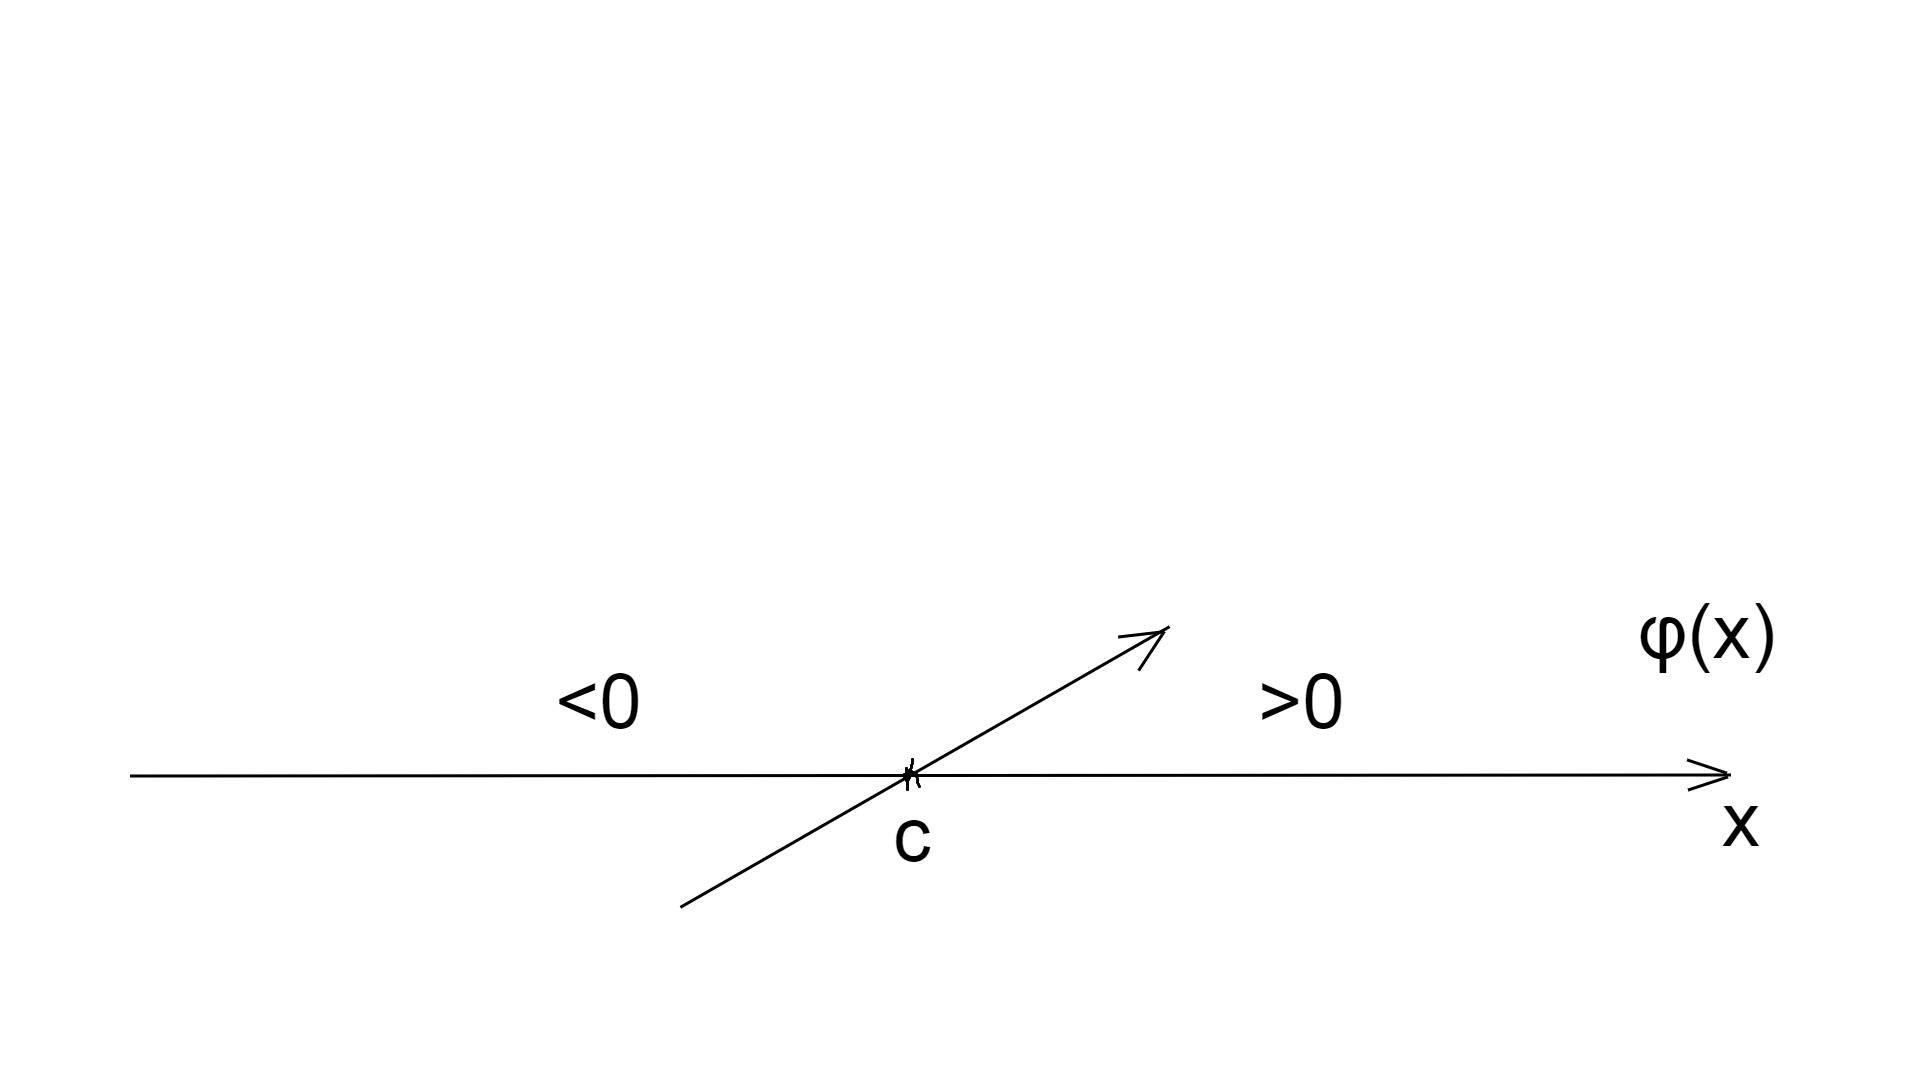
\includegraphics[trim={0 0 0 12cm}, clip, scale=0.08]{11_1_11_1.png}

\( \uparrow \) Так как \( y''(c)\ \exists \), то \( y'(x)\ \exists \) в некоторой окрестности точки \( x = c \). \( \varphi(x):\ \varphi(c) = 0, \varphi'(x) > 0 \) в \( x = c \). \( \Rightarrow \varphi(x) \) возрастает в \( x = c \).

Т.е. \( y'(x): \) при \( x < c:\ y'(x) < 0 \) и \( x > c:\ y'(x) > 0\ \xRightarrow[]{\textrm{Т. 3}} x = c \) --- точка локального минимума.

\textbf{Теорема 5.} Пусть \(y = f(x)\) непрерывна на \([a, b];\ y'\ \exists\) и непрерывна на \((a,b),\ \exists c\ :\ y'(c)=0;\ y''(x) > 0\) всюду на \((a,b)\), тогда \(x=c\) --- точка минимума \(y=f(x)\) на \([a,b]\)(если \(y''(x) < 0\), то \(x=c\) --- точка максимума на \([a,b]\)).

\( \uparrow \) Рассмотрим \( \varphi(x) = f'(x)\) 

\(\varphi(x): \begin{array}{l}
    \varphi(x)\ \textrm{--- непрерывна}\\
    \varphi(c) = 0\\
    \varphi'(x) > 0\ \textrm{на (a, b)}
\end{array}\)
\(\Rightarrow \varphi(x)\) возрастает на \((a,b)\), т.е. \(y'(x)\): при \(a < x < c\ y'(x) < 0\), т.е. \(y \searrow\);\\при \(b > x > c\ y'(x) > 0\), т.е. \(y \nearrow\)
\(\Rightarrow y(c)\) --- минимальное значение на \([a, b]\)

\textbf{Пример.} \( y = x^2 \)

\( (1) y' = 2x = 0 \Leftrightarrow x = 0 \)

\( (2) y'' = 2 > 0 \)

на промежутке \( [-1, 1] \)

Из $(1)$ или $(2)$ следует, что точка $0$ --- точка локального минимума.

\subsection{Направление выпуклости функции. Точки перегиба}

\textbf{Определение.} Если дуга \( y = f(x);\ a \leq x \leq b \) расположена не ниже касательной, проведенной в любой точке \(x \in (a, b)\), то \( y = f(x) \) называется \underline{выпуклой вниз} (по горбу) или \underline{вогнутая вверх} (по рогам) на \((a, b)\).

\textbf{Определение.} Аналогично, если не выше любой касательной, то \underline{выпуклая вверх}.

\textbf{Теорема.} Пусть \(y = f(x)\) непрерывна на \([a,b]\); и \(\exists f''(x)\) на \((a,b)\), если \(f''(x) > 0\) на \((a,b)\), то функция \(y = f(x)\) выпукла вниз на \((a,b)\)(если \(f''(x) < 0\), то выпукла вверх).

\(\uparrow\) Рассмотрим произвольную точку \( c \): \( a < c < x \leq b \). Проведем касательную в точке \( c: y_{\textrm{кас}} = f'(c)(x - c) + f(c) \). Рассмотрим вспомогательную функцию \( F(x) = y_{\textrm{крив}} - y_{\textrm{кас}} = f(x) - f(c) - f'(c)(x - c) \)

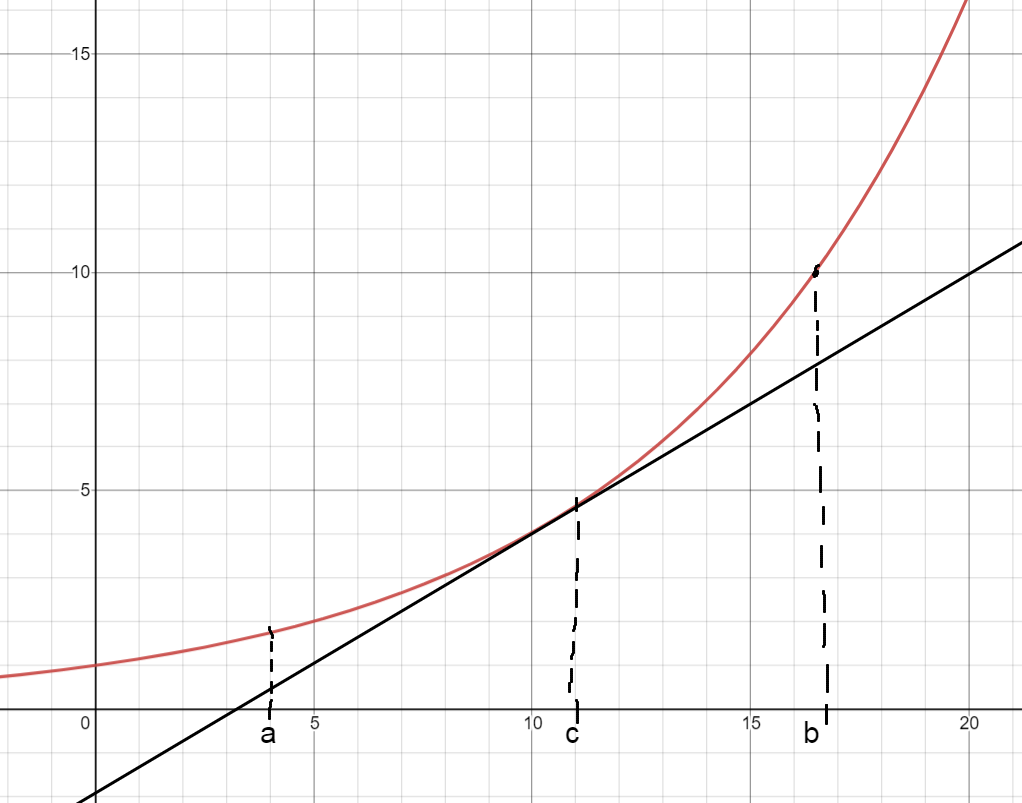
\includegraphics[scale=0.25]{11_1_11_2}

\( 
    \begin{array}{l}
        F(c) = 0\\
        F'(x) = f'(x) - 0 - f'(c) = f'(x) - f'(c)\\
        F'(c) = 0\\
        F''(x) = f''(x) - 0 = f''(x) > 0\\
        F''(c) = f''(c) > 0\\
    \end{array}
\xRightarrow[]{\textrm{Т. 5}} c \) --- точка минимума.

\( F(x) \) на \( [a; b] \)

\( F(x) \geq F(c) = 0 \) на \( [a; b] \), т.е. \( y_{\textrm{крив}} \geq y_{\textrm{кас}} \) в силу производности т. \(c\) функция \(y = f(x)\) выпукла вниз.

\textbf{Определение.} Точки О.О. функции \(y = f(x)\), в которых соединяются дуги с различной выпуклостью для \(f(x)\), называются точками перегиба.

Как найти точки перегиба.

\begin{enumerate}
    \item \( f''(x) \) на О.О.
    \item \( f''(x)=0\) или \(\nexists \Rightarrow\) подозрительные точки.
    \item Исследовать знак \( f''(x) \) слева и справа от подозрительных точек. При смене знака \( \Rightarrow \) точка перегиба.
\end{enumerate}

\textbf{Примеры:}

\begin{enumerate}
    \item \( y = x^4 - 6x^2 + 4 \)

    \begin{enumerate}
        \item \( t = x^2;\ t_{1, 2} = \frac{3 \pm \sqrt{9 - 4}}{1} \Rightarrow \) 4 корня.
        \item \(y' = 4x^3-12x = 4x(x^2 - 3) = 4x(x + \sqrt{3})(x - \sqrt{3})\)
        
        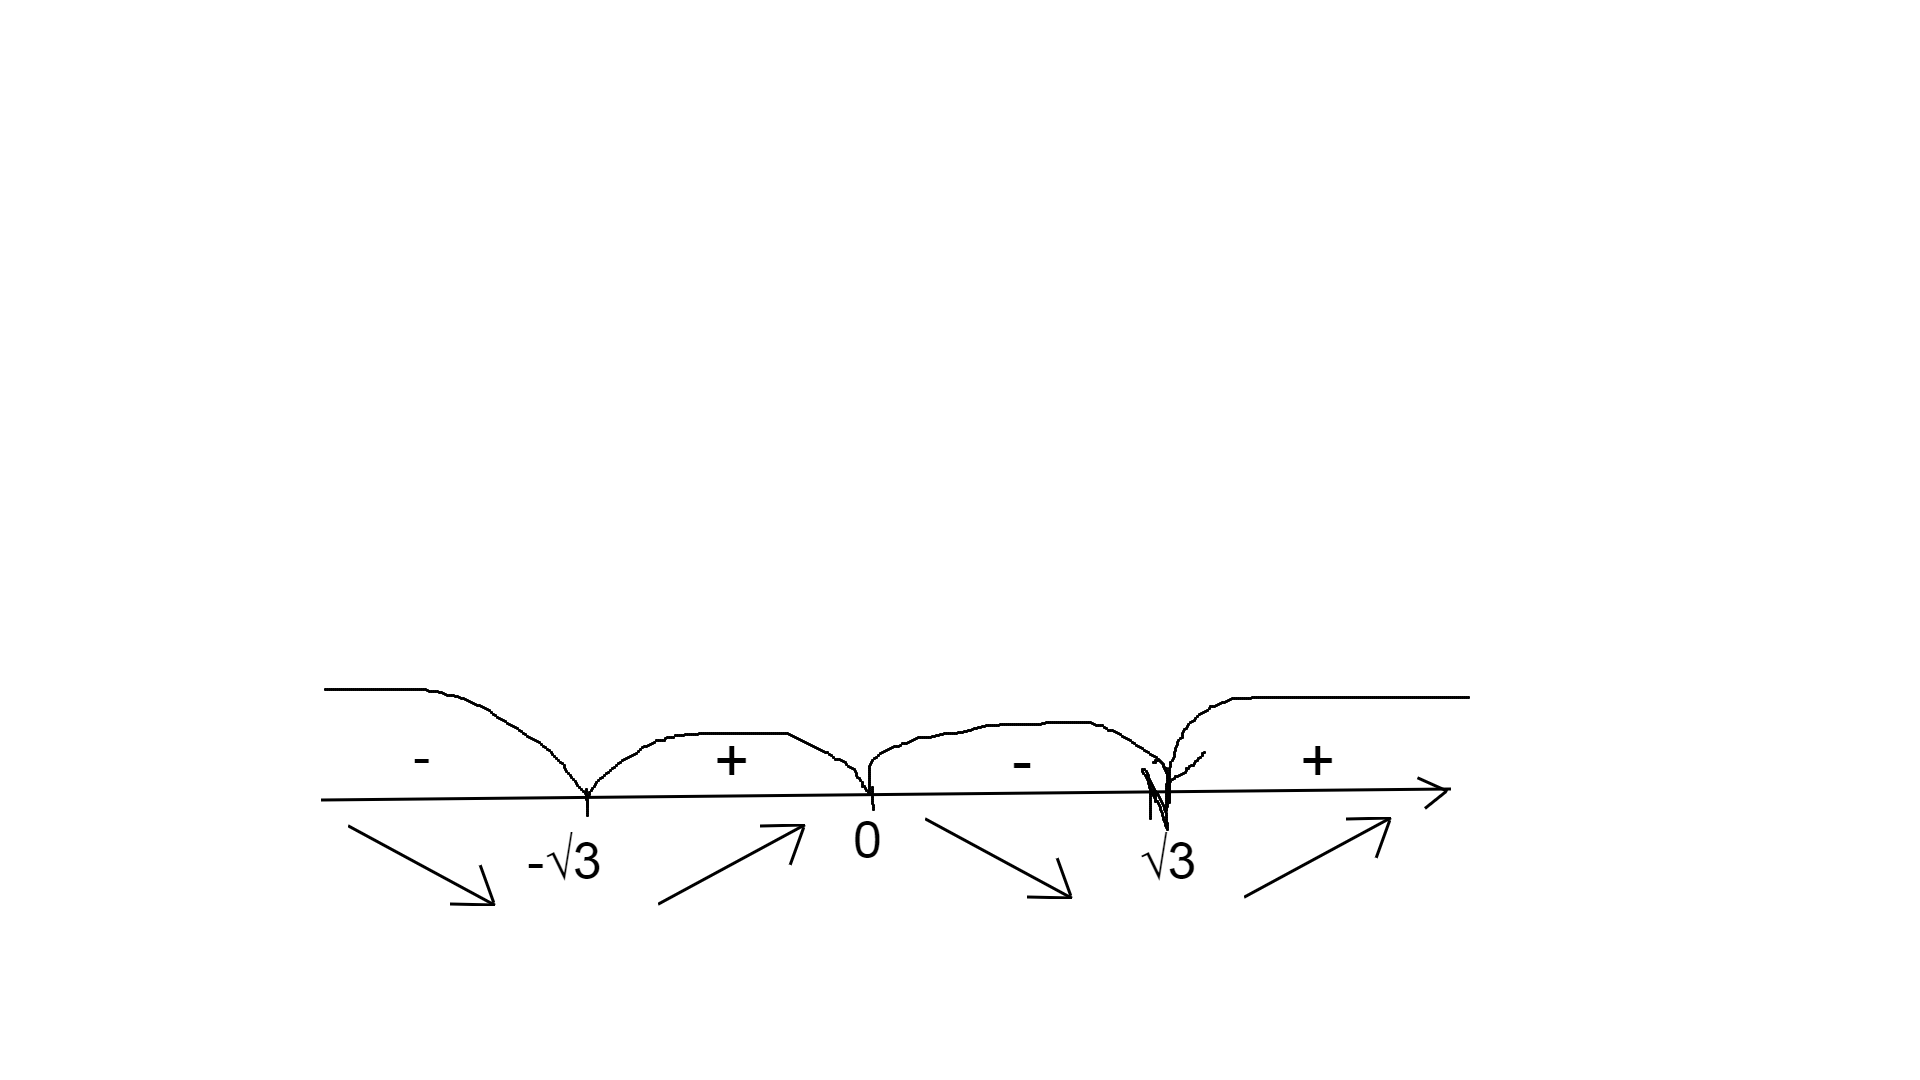
\includegraphics[trim={10cm, 5cm, 0, 20cm}, scale=0.15]{11_1_11_3.png}

        \( f(0) = 4 \)

        \( f(\pm \sqrt{3}) = 9 - 18 + 4 = -5 \)
        
        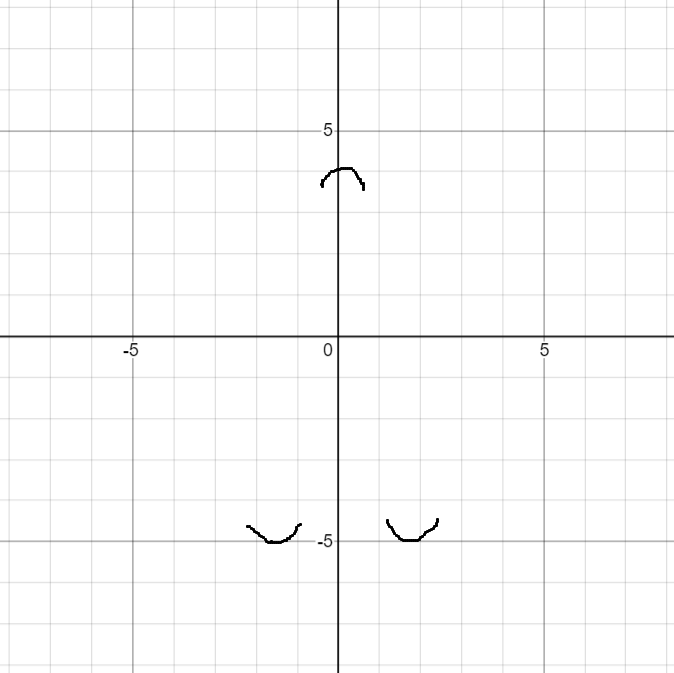
\includegraphics[scale=0.3]{11_1_11_4.png}

        \item \( y'' = 12x^2 - 12 = 12(x^2 - 1) = 12(x - 1)(x + 1) \)
        
        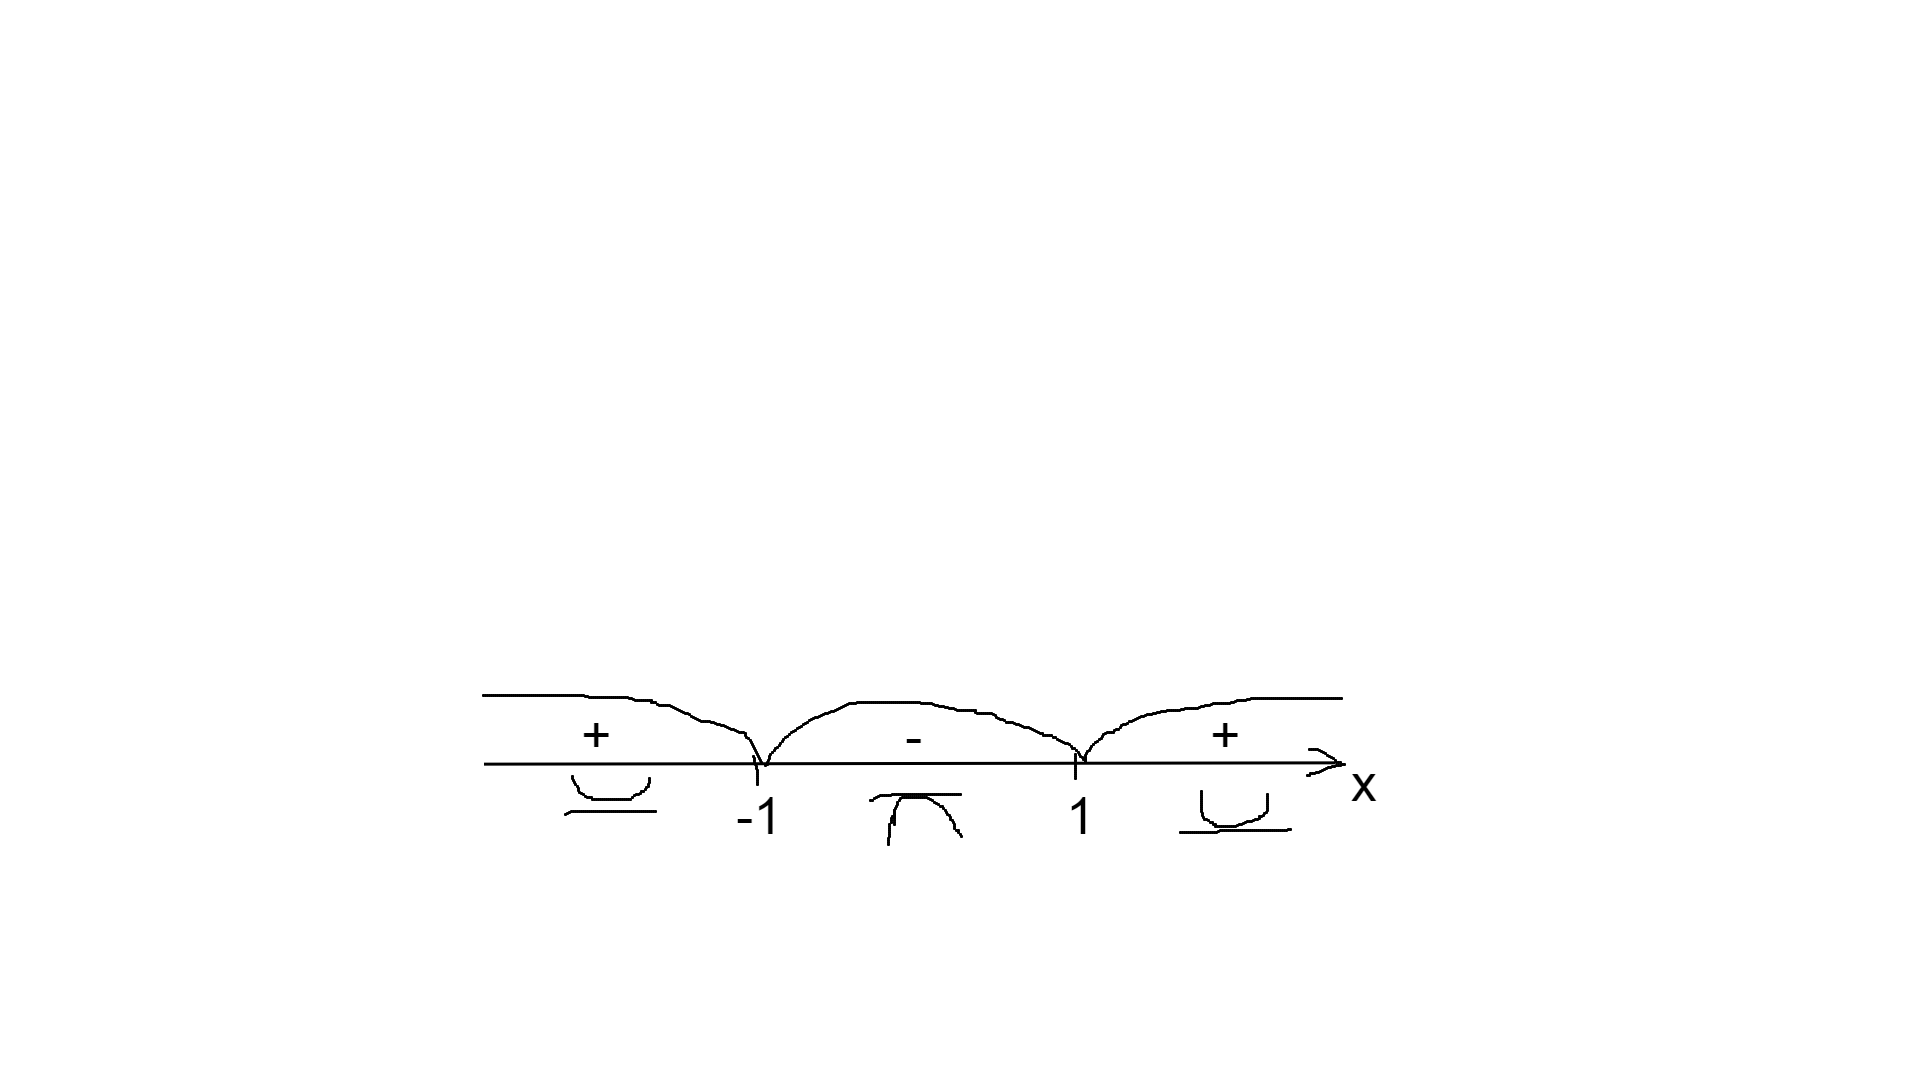
\includegraphics[trim={10cm, 5cm, 0, 20cm}, scale=0.15]{11_1_11_5.png}

        \( x = \pm 1\) --- точки перегиба.

        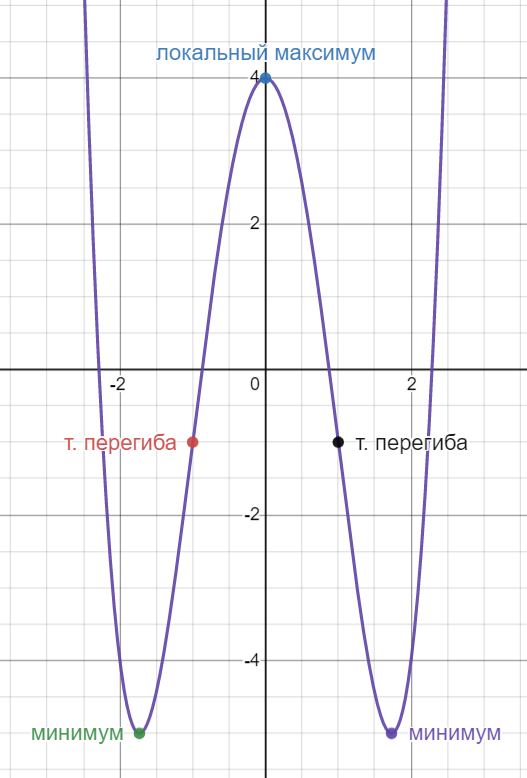
\includegraphics[scale=0.45, width=8cm]{11_1_11_6.png}

    \end{enumerate}
    \item \( y = \sqrt[3]{x} = x^{\frac{1}{3}} \)
    
    \begin{enumerate}
        \item О.О \( \forall x \).
        \item \(y = 0 \Leftrightarrow x = 0\).
        \item \( y' = \frac{1}{3}x^{-\frac{2}{3}} = \frac{1}{3}\frac{1}{x^{\frac{2}{3}}} \)
        \item \( y''(x) = \frac{1}{3}(-\frac{2}{3})x^{-\frac{5}{3}} = -\frac{2}{9}\frac{1}{x^{\frac{5}{3}}} \)
        \( x = 0 \) --- точка перегиба.
    \end{enumerate}
\end{enumerate}

\textbf{Замечание.} Если первая производная в точке перегиба существует, то функция пересекает касательную, проведённую в этой точке.

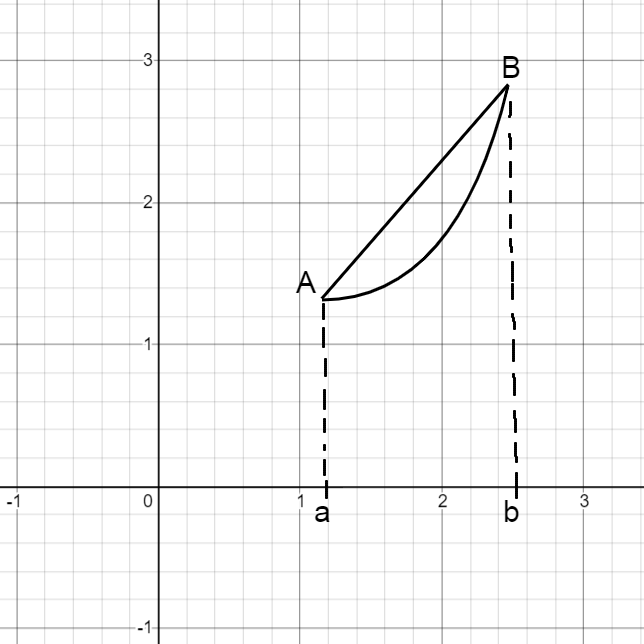
\includegraphics[scale=0.3]{11_1_11_7.png}

\textbf{Теорема.} Если \( y = f(x) \) на промежутке \( [a, b] \) выпукла вниз, то \( \forall x \in [a, b]: f(x) \) расположена не выше хорды \(AB\). (аналогично для выпуклых вверх)

\(\uparrow\) Рассмотрим произвольную точку \(c \in (a,b)\) и касательную в этой точке.

Т.к. функция выпукла вниз, то \(A\) не ниже \(A_1\), а точка \(B\) не ниже \(B_1\).

\(\Rightarrow\ \forall\) точек отрезков \(A_1B_1\) и \(AB\) будет аналогичное свойство; т.е. \(M_1\) не выше \(M\ \Rightarrow\) ч.т.д. в силу произвольности т. \(c\ \downarrow\)

Т.е. \(\approx f(c) \leq y_{\textrm{хорды}}\)

Если выпукла вниз, то \(\Rightarrow f(\frac{a+b}{2}) \leq \frac{f(a)+f(b)}{2}\)

\(\Rightarrow (x, y \geq 0), (\frac{x+y}{2})^3 \leq \frac{x^3 + y^3}{2}\).

\(c = a +\theta(b - a) = (1 - \theta)a + \theta b,\ 0 < \theta < 1\)

\subsection{Схема исследования функции}

\begin{enumerate}
    \item О.О. и исследование функции на границах О.О.
    \item Четность.
    \item Периодичность.
    \item Нули и промежтуки знакопостоянста.
    \item Точки экстремума и промежутки возрастания и убывания.
    \item Промежутки вогнутости, выпуклости и перегиба.
    \item Асимптоты.
    \item Особенности графика(максимумы, минимумы).
\end{enumerate}

\subsection{Асимптоты графика функции}

\textbf{Определение.} Если функция определена на интервале \( (a, b) \) и \( \lim_{x \to a+0} f(x) = \infty \), то \( x = a \) называется вертикальной асимптотой для \( y = f(x) \) в \( x = a \) справа.

Аналогично, если \(\lim_{x \to b-} f(x) = \infty\), то \(x = b\) --- вертикальная асимптота при \(x = b\) слева.

\textbf{Пример.} \( y = \frac{1}{x} \)

О.О: \( x \neq 0 \), т.е. \( x in (-\infty; 0) \cup (0; +\infty) \)

\( \lim_{x \to 0-} \frac{1}{x} = -\infty \)

\( \lim_{x \to 0+} \frac{1}{x} = +\infty \) 

\( \Rightarrow x = 0 \) --- вертикальная асимптота.
\end{document}
